\section{Convex Hull Algorithms}

\subsection{\textbf{Brute Force Convex Hull:}}

The Brute Force algorithm exhibits high time complexity, making it impractical for large datasets. The resulting convex hull may be accurate, but the computational cost is significant.

\begin{figure}[h]
    \centering
    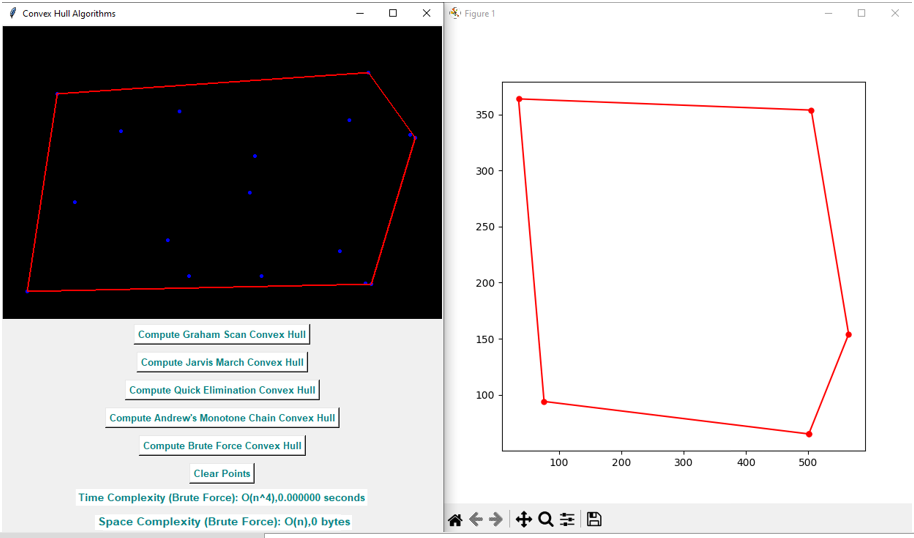
\includegraphics[width=1\linewidth]{bruteforce imsge.PNG}
    \caption{Brute Force}
    \label{fig:bruteforce}
\end{figure}

\vspace{10pt} 

\subsection{\textbf{Jarvis March Convex Hull:}}

Jarvis March provides a simple and intuitive solution with moderate time complexity. However, it may struggle with degenerate cases.

\begin{figure}[h]
    \centering
    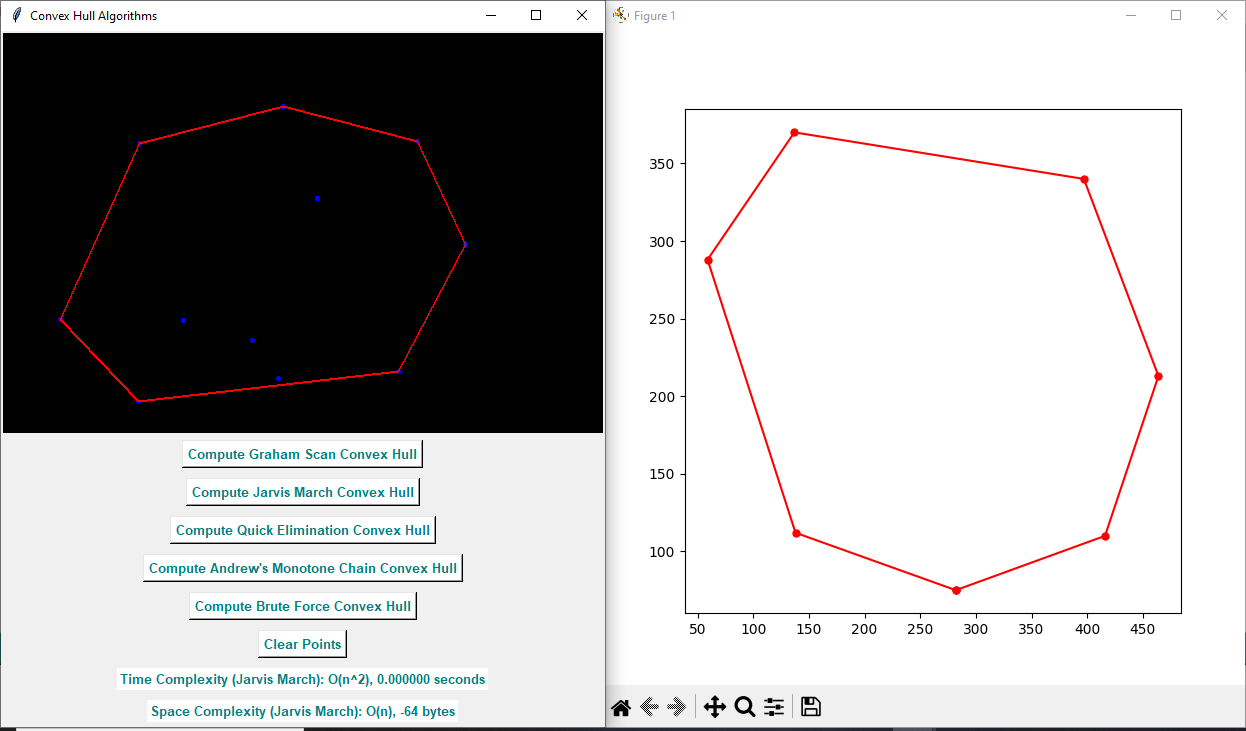
\includegraphics[width=1\linewidth]{jarvis.PNG}
    \caption{Jarvis March}
    \label{fig:jarvis}
\end{figure}

\vspace{10pt}

\subsection{\textbf{Graham Scan Convex Hull:}}

Graham Scan demonstrates improved efficiency, especially for large datasets. Its sorting step contributes to better overall performance.

\begin{figure}[h]
    \centering
    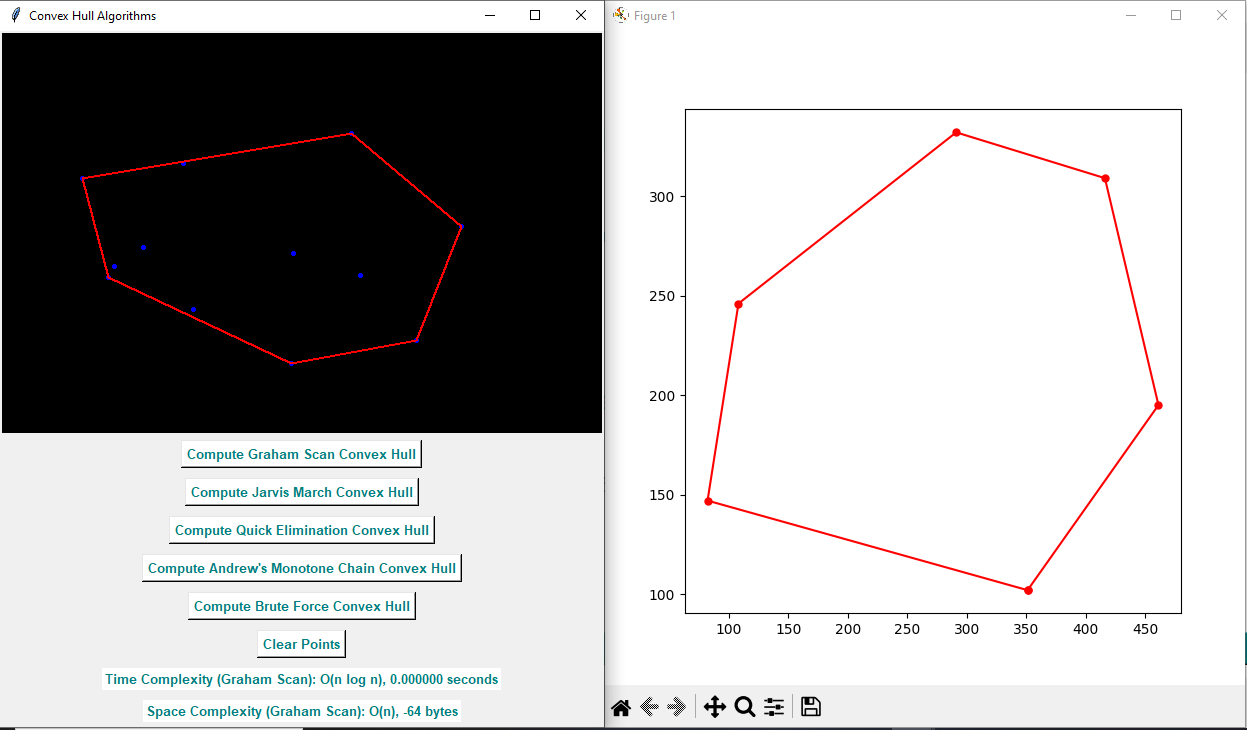
\includegraphics[width=1\linewidth]{grahamscan.PNG}
    \caption{Graham Scan}
    \label{fig:grahamscan}
\end{figure}

\vspace{10pt}



